\documentclass[12pt]{article}
\usepackage{amsmath,amsfonts, epsfig}
\usepackage{booktabs} % for better table formatting
\usepackage{array}
\usepackage{multirow}
\usepackage{graphicx}
\usepackage{fancyhdr}
\usepackage{bm}
\pagestyle{fancy}
\lfoot{\texttt{ematm0067.github.io}}
\lhead{Introduction to AI - 04.1\_k-means - Conor}
\rhead{\thepage}
\cfoot{}

\usepackage{tikz}
\usetikzlibrary{positioning}

\usetikzlibrary{shapes.misc}


\usepackage{ifthen,calc}
\newboolean{nopics}
\setboolean{nopics}{false}


\begin{document}

\section*{Unsupervised and supervised learning}

In the Hawks data set, which is available as part of the Stat2Data
library in R and is copied in the unit github, wing and weight measurements are made for three types of hawk:\\
\\
CH=Cooper's, RT=Red-tailed, SS=Sharp-Shinned\\
\\
with a pretty unequal distribution:
\begin{center}
  
\begin{tabular}{l|cccc}
  &CH&RT&SS&total\\
  \hline
  number&31&121&68&221
  \end{tabular}
\end{center}
We can plot this data and the result is shown in Fig.~\ref{fig:hawks_plot}. Obviously supervised learning works in this case and this would be useful if we found a hawk and didn't know how to identify it; from the decision boundaries we can see that knowing the wing length and weight would allow us to identify the hawk.

\begin{figure}[htb]
\begin{center}  
  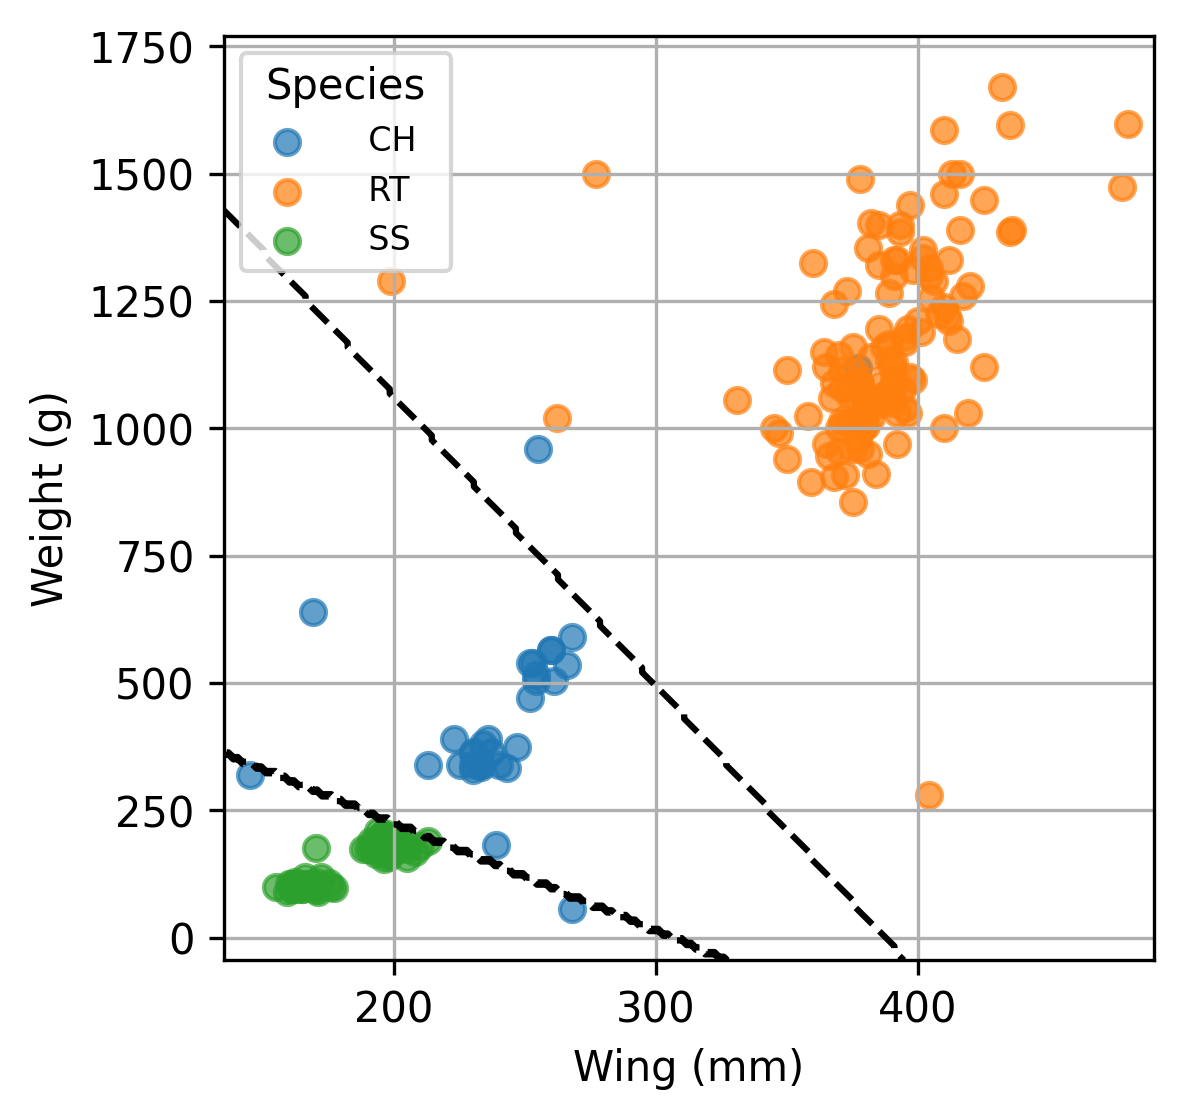
\includegraphics{hawks_plot.png}
\end{center}
\caption{The hawk data is plotted with wing length and weight; the three species have been marked by colour. Clearly the three species correspond to different clusters and logistic regression has been used to find the two decision boundaries plotted as black dashed lines, these are pretty accurate.\label{fig:hawks_plot}}
\end{figure}

In this case we are clearly benefiting from the expertise of the
people who supplied the data. The machine learning algorithm isn't
doing something new for us, it isn't working out how many different
types of hawks there are, or discovering stuff we didn't know; instead
it is allowing us to apply to new data points, new hawks, a
classification we have already discovered. This seems a less important
task than the \textsl{unsupervised} task, to classify without being
told the classes. Say you just went out an measured some hawks and had
the results in Fig.~\ref{fig:hark_unlabel}, could you spot that there were species.


n\begin{figure}[htb]
\begin{center}  
  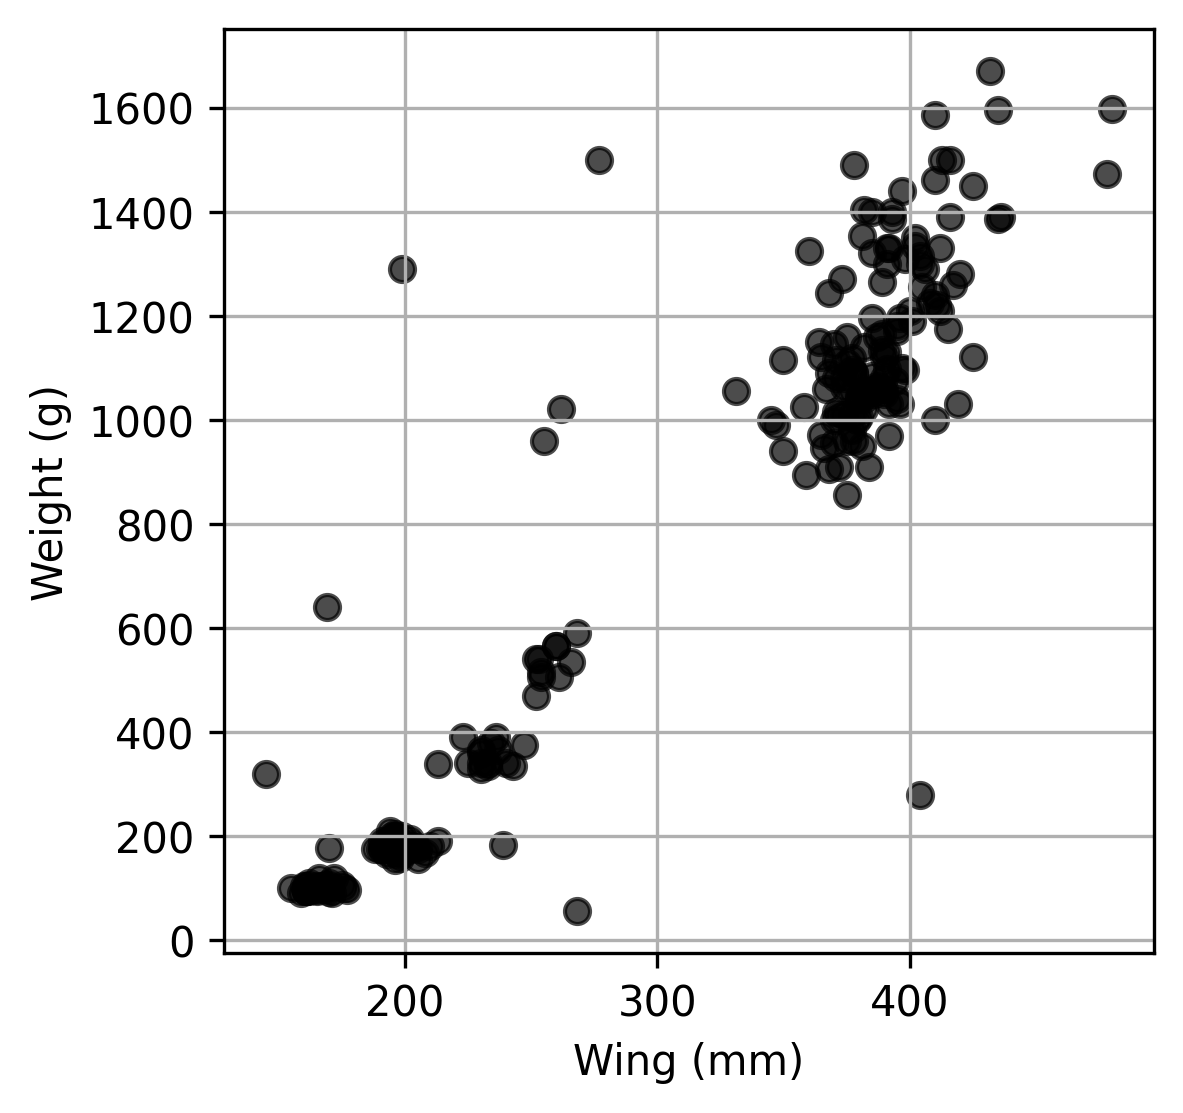
\includegraphics{hawks_plot_unlabel.png}
\end{center}
\caption{The hawk data is plotted with wing length and weight but without labels, it isn't so clear that there should be three clusters, it looks more like five or six, maybe the sex of the hawks also has an affect. Unsupervised learning is hard!\label{fig:hawks_unlabel}}
\end{figure}

Unsupervised learning, studying unlabelled data, is about discovering
structure in the data. Clearly this is useful and hard and in an
obvious way its goal is discovering knowledge, rather than applying
it. We should not take too seriously this stark division between
supervised and unsupervised learning, for a start it relies on an
obvious division between ``label'' and other properties of the
data. These days it feels like training and learning approaches often
combine supervised and unsupervised elements, along, indeed, with
reinforcement learning. Here we will look at some unsupervised
learning algorithms, they give a lot of insight.

\section*{$k$-means clustering}

Probably the most famous and the most straight-forward approach to
unsupervised learning is $k$-means; $k$-means only works in very
specific situations but it is always the first thing to try. In
$k$-means you decide how many clusters you think there should be, that
doesn't sound very `unsupervised', but in practice given how quickly
the algorithm runs, you can try different values. $k$ different points
are picked at random, these are the \textsl{centroids} and to each $k$
points the data points that are nearer to it than to any of the other
centroids is given to that centroid. That gives $k$ sets of points, one
for each centroid. Now $k$ new centroids are calculate, each is at the
center of a cluster. This is then repeated until the centroids stop moving.

In mathematics here it is the algorithm again, let
\begin{equation}
  \mathcal{D}\{\mathbf{x}_1,\mathbf{x}_2,\ldots,\mathbf{x}_n\}
\end{equation}
be the data and $\mathbf{y}_1$ up to $\mathbf{y}_k$ be the initial centroids. Now make the clusters
\begin{equation}
  C_i=\{\mathbf{x}_j\in\mathcal{D}:d(\mathbf{x}_j,\mathbf{y}_i)<d(\mathbf{x}_j,\mathbf{y}_{i'})\forall i'\not=i\}
\end{equation}
where $d(\mathbf{x},\mathbf{y})$ is the distance between $\mathbf{x}$ and $\mathbf{y}$; usually this would just be the Euclidean distance:
\begin{equation}
  d(\mathbf{x},\mathbf{y})=|\mathbf{x}-\mathbf{y}|
\end{equation}
and we will discuss the choice of distance later\footnote{In this set
up with the Euclidean distances there are unlikely to be draws, but if
there are draws you need a procedure for dealing with them. This is
usually just fiddly but not a problem!}. Now you make new centroids:
\begin{equation}
  y_i\rightarrow \frac{1}{|C_i|}\sum_{\mathbf{x}_j\in C_i}\mathbf{x}_j
\end{equation}
and repeat.

Lets try it with the hawk data; in Fig.~\ref{fig:khawks}. The
algorithm converges quickly and gives three clusters, just not the
clusters we might've expected. This is the thing with unsupervised
learning, it learns from the data, not our intuition. If we were
hoping to discover hawk species this way we would fail, it clusters
together the CT and SS hawks and splits the RT into two. However, we
also learn something, we learn that this is what the unsupervised
algorithm sees and as data scientists we'd consider if we had the
correct value of $k$. In Fig.~\ref{fig:khawksk6} we use $k=6$ and get
something more like we might expect. Hopefully this shows the
advantages and the disadvantages of using $k$-means, we started off
hoping to discover species using the clustering, in the end we learned
that weight and wing length does not produce natural clusters
corresponding to species and we had to use our intuition to suggest we
need to look at other properties as well.

In the next note we will think a bit more about how to pick $k$ and to
assess the quality of our clustering once we have performed it. The
main point is that $k$-means works best when the clusters are
spherical and roughly equal; obviously the Hawks data has clusters
that are neither very spherical nor of equal size, though making a
smaller data set with the same number of each hawk doesn't help,
unsupervised learning still doesn't give clusters corresponding to the
three hawk types, though, and this is the important point, it does
tell you something about the data.

\begin{figure}[htb]
\begin{center}  
  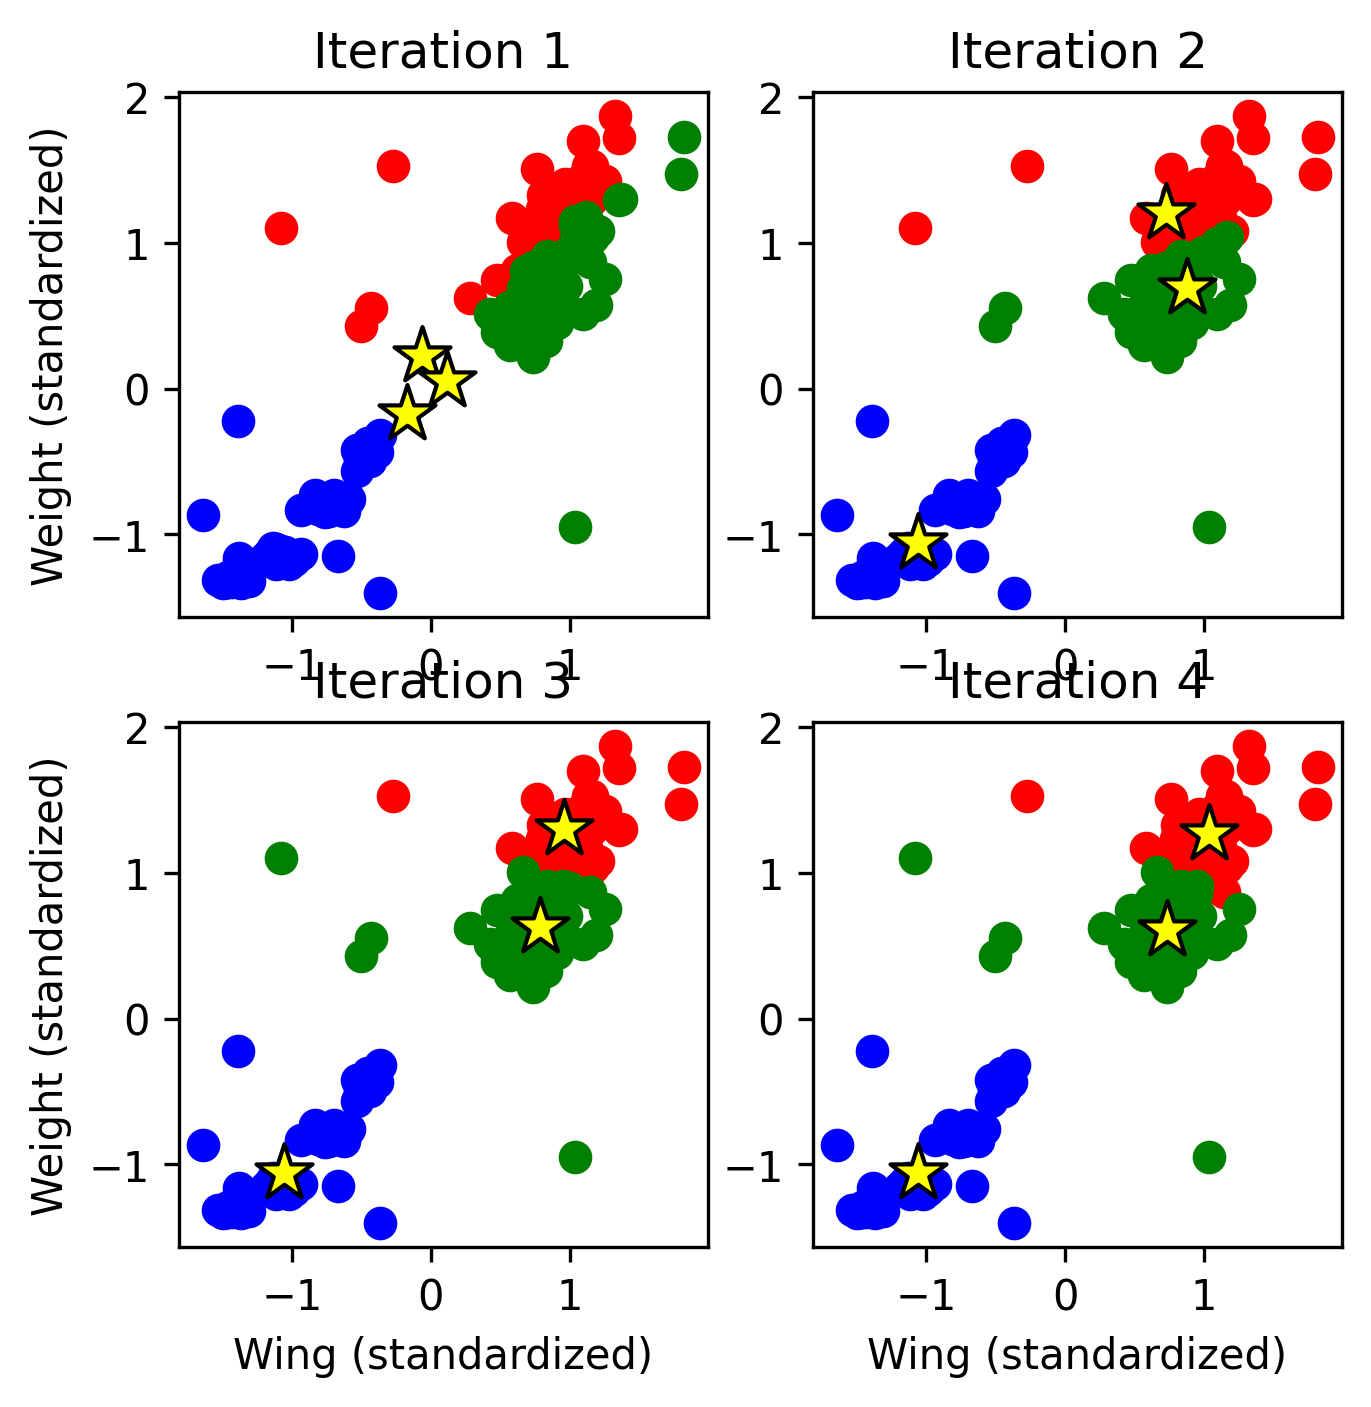
\includegraphics{04.1_khawks.png}
\end{center}
\caption{The $k$-means algorithm is run for the hawk data with
  $k$=3. This uses standarded values for the two component values,
  wing length and weight; because the two things aren't really
  comporable, one measured in milimeters, the other in grammes, it
  would be peculiar to just measure distances in the mixed gram,
  milimeter space. Instead we standardize first, take away the mean
  and divide by the standard deviation, now the two components have no
  units and have a similar spread of values. The first values are
  randomly chosen near the middle to make it easier to see what's
  happening, usually we just pick $k$ of the points as the initial
  centroids.\label{fig:khawks}}
\end{figure}


\begin{figure}[htb]
\begin{center}  
  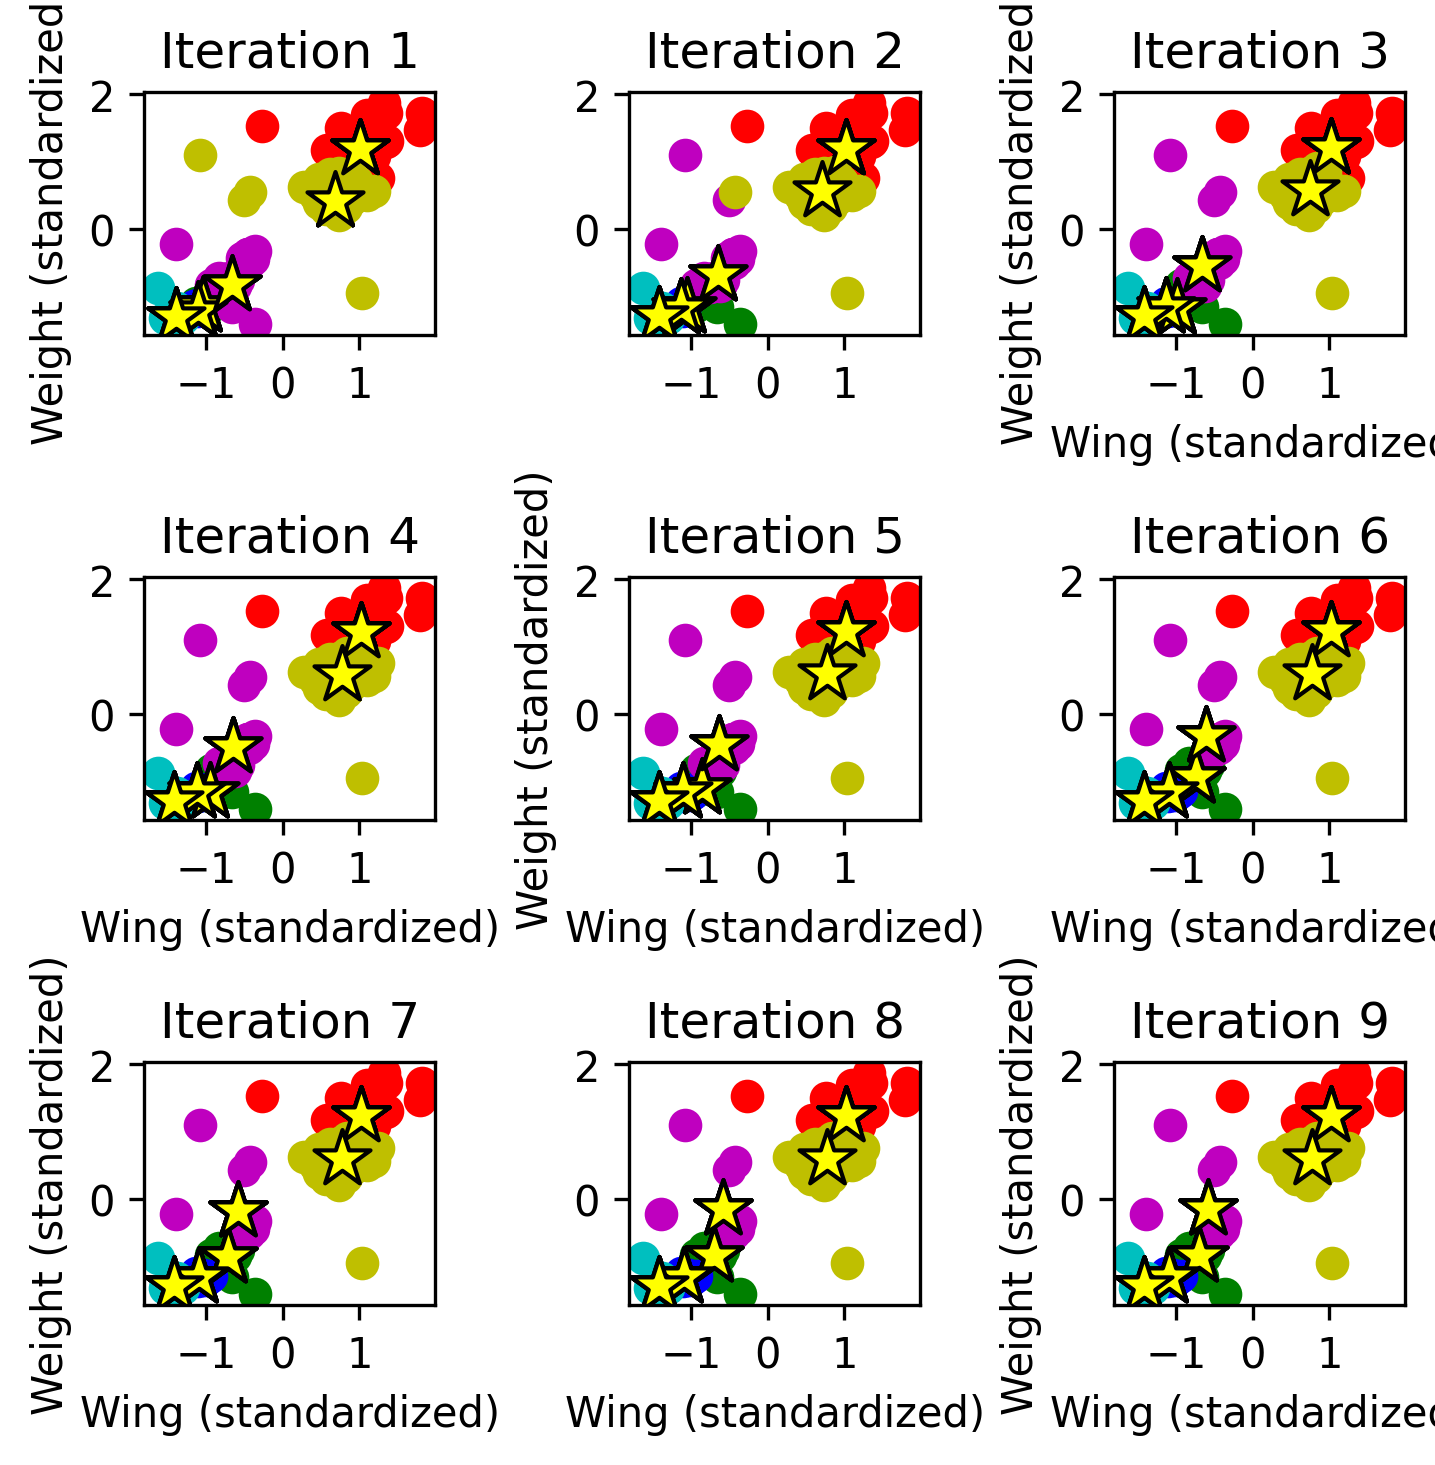
\includegraphics{04.1_khawks_k6.png}
\end{center}
\caption{The $k$-means algorithm is run for the hawk data with
  $k$=6. This takes longer to converge, but iteration 9 is actually
  the same as iteration 8; I included it just to make up the grid. It
  has found six clusters, roughly two for each of the species we saw
  at the start, probably corresponding to each of two
  sexes..\label{fig:khawksk6}}
\end{figure}

\subsection*{A few final comments!}

One nice thing about the $k$-means algorithm is that it always
converges, after a finite number of steps it will find the same
centroids as in the previous iteration and halt. The thing that isn't
so good is that it doesn't always stop at the same place, there is
some depedence on the initial condition. Often, the algorithm will be
run several times from different starting points to try to find the
best clustering, we will return to the notion of best clustering in
the next section, but, roughly, if
\begin{equation}
  \mathcal{C}=\{C_1,C_2,\ldots,C_k\}
\end{equation}
is a set of clusters  with corresponding centroids $\mathbf{c}_i$ then one the degree of dissimilarity
\begin{equation}
  J(\mathcal{C})=\sum_{i=1}^k\sum_{\mathbf{x}_j\in C_i}[d(\mathbf{x}_j,\mathbf{c}_i)]^2
\end{equation}
measures how good the clustering is; the lower the better, so the idea
of multiple restarts is to run the algorithm a few times and pick the
clustering with the lowest $J(\mathcal{C})$. In fact,
Fig.~\ref{fig:khawks_different_starts} shows that $k$-means sometimes
produces the `correct' clustering for our hawk data.


\begin{figure}[htb]
    \begin{tabular}{ll}
      \textbf{A}&\textbf{B}\\
      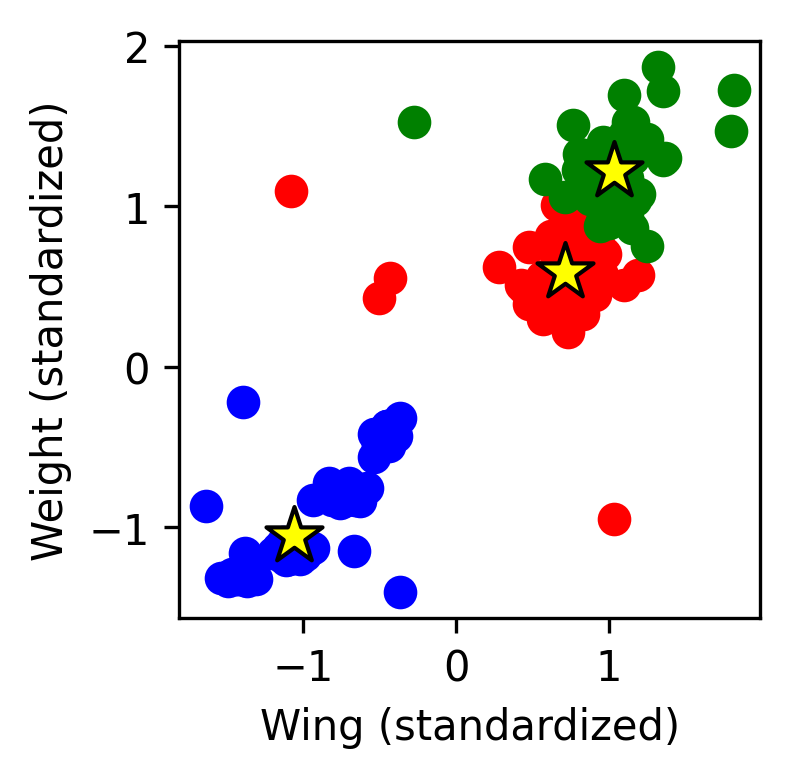
\includegraphics{04.1_khawks_142.png}&
      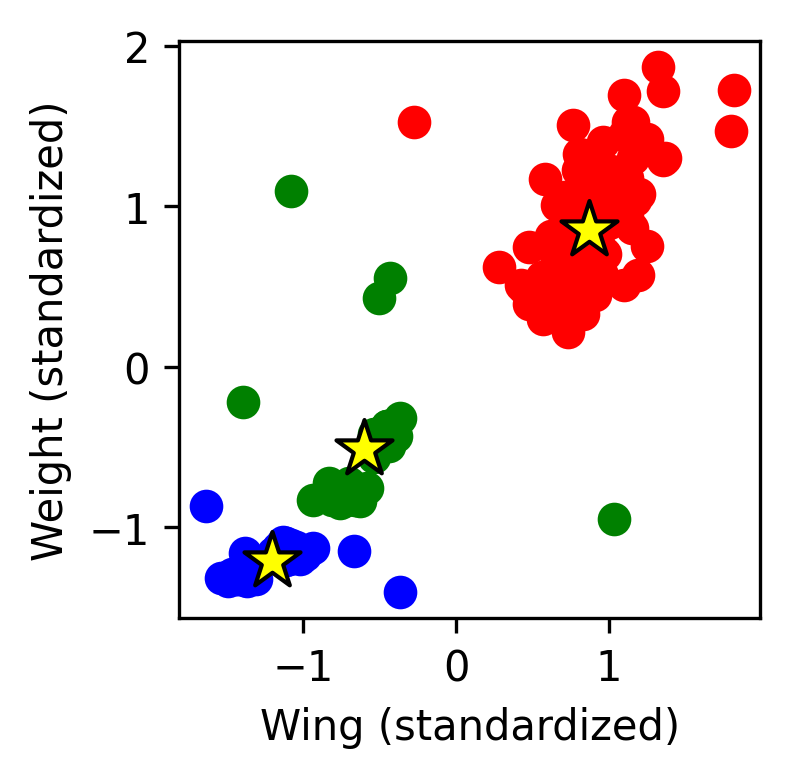
\includegraphics{04.1_khawks_42.png}
    \end{tabular}
    \caption{Here the initial conditions are chosen differently for
      the $k$-means algorithm, \textbf{A} shows the same behaviour we
      have seen before, splitting the RT's into two clusters and
      making one cluster out of CH and SS; \textbf{B} on the other
      hand comes close to having a cluster for hawk type. The quantity
      $J$ his nearly the same for each, $J=37.27$ for \textbf{A} and
      $J=37.31$ for \textbf{B}, showing that the difference between
      the unsupervised clustering and the clusters based on species is
      not a result of the algorithm not finding the solution reliably,
      it reflects the fact that the clustering is, itself, ambiguous,
      there are two different, equally good, clusterings as far as
      $k$-means is concerned!
\label{fig:khawks_different_starts}}
\end{figure}



Mostly we have been thinking about using the Euclidean distance
function here, of course, the choice of distance is important and the
method only works in so far as the distance represents difference. In
the examples above we used standardised distances in an attempt to
match up the notion that the differences in the weight and the
differences in the wing length where somehow comparable, even if one
is measured in grammes and the other in milimeters. We then put them
together like so
\begin{equation}
  d(\textbf{x},\textbf{y})=|\textbf{x}-\textbf{y}|=\sqrt{\sum_i (x_i-y_i)^2}
\end{equation}
but there are other ways that this can be done; for example you could
use the Manhattan or $L^1$ metric\footnote{These are two names for the
same thing, this distance is called the Manhattan metric because, as
explained in the next paragraph, it resembles travel in a city with a
grid system, it is called $L^1$ because it is part of a family of metrics, the $L^p$ metrics where $p=2$ corresponds to the Euclidean distance.}.
\begin{equation}
  d_1(\mathbf{x},\mathbf{y})=\sum_i |x_i-y_i|
\end{equation}
In one way all this choice, the choice of $k$ we discuss in the next
note, the choice of metric, makes $k$-means a slippery sort of
technology; it is not very good a \textsl{proving} things, conversely
it is useful for discovering things because you can try different
stuff, see what works and then try to understand why that worked.

Why would the Manhattan distance be better in some situations. It all
depends on where the structure is in relationships. Imaging have
information about lots of people living in Manhattan, north of the
Village, where the grid system is rigid, all the roads run north-south
or east-west. Imagine you thought that by clustering people by how far
they lived from each other you could find neighbourhoods, obviously
the appropriate metric is the $L^1$ metric since that determined how
far one person is from another in walking distance, the Euclidean, as
the crow flies, distance is irrelevant!

There are situations where you can measure a distance between two
data-points even if they don't live in some sensible space. An example
might be something like this: imagine you want to investigate coffee,
you want to see if there are clusters of different coffee types. You
could get a lot of tasters and test to see if they are able to
distinguish between pairs of coffee, you can ask the tasters for each
pair ``are these two samples from the same beans or different
beans?'', sometimes doing this when the beans are the same so the
question is genuine. Now you could define the distance between two
types of beans as the number of people who said ``different'' in the
task above. Now, although you have distances between beans, you don't
have space they live in, you can't work out a centroid for a cluster
because you can't add or divide coffee beans, only vectors. In this
case you can use the $k$-medoids algorithm, the idea here is to
replace the centroid with the \textsl{medoid}, the `middle-est' point in
the cluster. For each point in a cluster $C_i$ you can get a score $M$
\begin{equation}
  M(C_i,\textbf{x})=\sum_{\mathbf{y}\in C_i} d(\mathbf{x},\mathbf{y})
\end{equation}
where $\mathbf{x}\in C_i$. The medoid is now the point that has the smallest value of $M$.






\end{document}

